\documentclass{cours}
\usepackage{pgfplots}
\usepackage{multicol}
\usepackage{amssymb}
\usepackage{xr}
\usepackage{fontawesome}
\usetikzlibrary {decorations.text, backgrounds, intersections}
\usepackage{mhchem}

\externaldocument[]{18-premier_principe}
\begin{document}


\setcounter{chapter}{20}
\chapter{Machines thermiques}

Dans ce chapitre, nous allons appliquer les principes de la thermodynamique aux machines thermiques. Une machine thermique décrit n'importe quel système thermodynamique qui subit une transformation cyclique en échangeant du travail et de la chaleur avec le milieu extérieur.


\section{Exemples de machines thermiques}%
\label{sec:exemples_de_machines_thermiques}

\subsection{Le moteur à vapeur}%
\label{sub:le_moteur_a_vapeur}
Un moteur à vapeur est une machine qui a pour objectif de convertir une énergie thermique produite dans une chaudière en travail. Le travail fourni pouvait servir autrefois à faire avancer des trains, aujourd'hui il sert principalement à produire de l'électricité.

Le principe de fonctionnement est le suivant :
\begin{itemize}
  \item De l'eau liquide est chauffée dans la chaudière pour produire de la vapeur sous pression ;
  \item la vapeur produite fait tourner une turbine qui fournit au milieu extérieur (générateur électrique) un travail mécanique ;
  \item la vapeur est liquéfiée dans un condenseur ;
  \item l'eau liquide est renvoyée vers la chaudière pour démarrer un nouveau cycle.
\end{itemize}

\begin{center}
  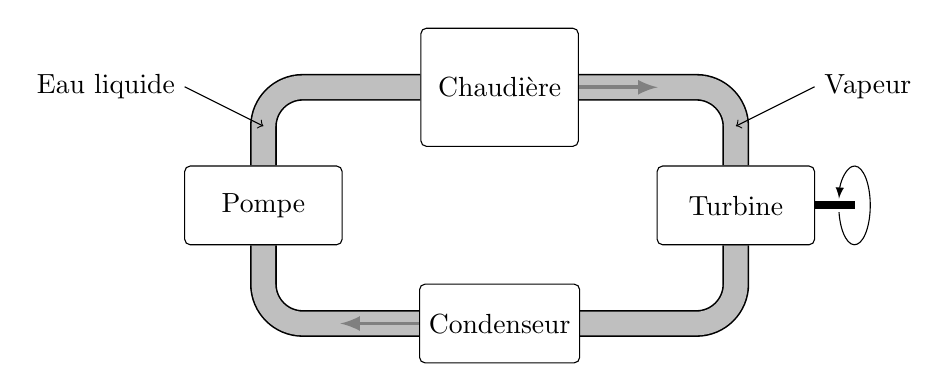
\begin{tikzpicture}
    %tikz thermo
\tikzset{
    partial ellipse/.style args={#1:#2:#3}{
        insert path={+ (#1:#3) arc (#1:#2:#3)}
    }
}

    \node[minimum width=2cm, minimum height=1cm, rounded corners=2pt, draw](Pompe) at (0,0) {Pompe}; 
    \node[minimum width=2cm, minimum height=1.5cm, rounded corners=2pt, draw](Chaudiere) at (3,1.5) {Chaudière}; 
    \node[minimum width=2cm, minimum height=1cm, rounded corners=2pt, draw](Turbine) at (6,0) {Turbine}; 
    \node[minimum width=2cm, minimum height=1cm, rounded corners=2pt, draw](Condenseur) at (3,-1.5) {Condenseur}; 
    \begin{scope}[on background layer]
    \draw[line width=3mm, rounded corners=5mm, gray!50, preaction={draw, line width=3.4mm, black}] 
     (Pompe.north) |- (Chaudiere.west) 
     (Chaudiere.east) -| (Turbine.north)
     (Turbine.south) |- (Condenseur.east)
     (Condenseur.west) -| (Pompe.south);
     \draw[-latex, line width=0.5mm, gray] (Condenseur.west) -- ++(-1, 0);
     \draw[-latex, line width=0.5mm, gray] (Chaudiere.east) -- ++(1, 0);
     \draw[line width=1mm] (Turbine.east) --++(0.5,0);
     \draw[-latex] (Turbine.east) ++(0.5,0) [partial ellipse=190:530:0.2cm and 0.5cm];
    \end{scope}
    \draw[<-] (Pompe.north)++(0, 0.5) -- ++(-1, 0.5) node[left]{Eau liquide};
    \draw[<-] (Turbine.north)++(0, 0.5) -- ++(1, 0.5) node[right]{Vapeur};
  \end{tikzpicture}
  \captionof{figure}{Principe d'un moteur à vapeur}
\end{center}

Nous modéliserons le système de la manière suivante : 
\begin{itemize}
  \item Le système thermodynamique $\Sigma$ est une mass $m$ d'eau ;
  \item La chaudière est la \textbf{source chaude} à la température $T_c$ qui fournit une quantité de chaleur $Q_c>0$ au système ;
  \item Le condenseur est la \textbf{source froide} à la température $T_f$ qui fournit une quantité de chaleur $Q_f<0$ au système ;
  \item La pompe fournit un travail $W_p>0$ au système ;
  \item La turbine fournit un travail $W_t<0$ au système (c'est le système qui lui fournit du travail).
\end{itemize}
\begin{minipage}{\linewidth}
\begin{center}
  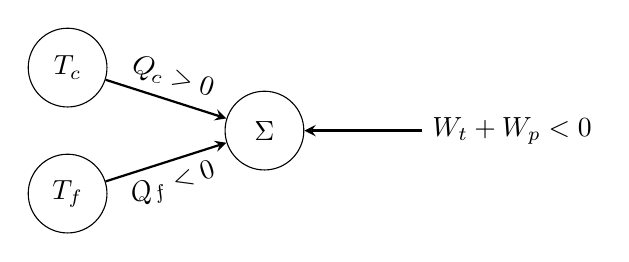
\begin{tikzpicture}
    %tikz thermo
    \node[circle, draw, minimum width=1cm] at (-2.5, 0.8) (Tc){ $T_c$ };
    \node[circle, draw, minimum width=1cm] at (-2.5, -0.8) (Tf){ $T_f$ };
    \node[circle, draw, minimum width=1cm] at (0,0) (S){ $\Sigma$ };
    \draw[-stealth, thick] (Tc) -- node[above,sloped]{ $Q_c>0$ }(S);
    \draw[-stealth, thick] (Tf) -- node[below, sloped]{ $Q_f<0$ }(S);
    \draw[stealth-, thick] (S) --  ++(2, 0)node[right]{ $W_t+W_p<0$ };
  \end{tikzpicture}
\captionof{figure}{Modélisation de la machine à vapeur}
\end{center}
\end{minipage}
La machine à vapeur est un \textbf{moteur ditherme}, c'est un moteur (fournit du travail au milieu extérieur) qui fonctionne en échangeant de la chaleur avec deux thermostats. 

\subsection{Le réfrigérateur}%
\label{sub:le_refrigerateur}
Un réfrigérateur est une machine dont l'objectif est de refroidir. En pratique, on procède de la manière suivante :
\begin{itemize}
  \item Un \textbf{compresseur} comprime un fluide sous forme de gaz, lors de la compression, le gaz s'échauffe au dessus de la température ambiante ; 
  \item le gaz chauffe circule dans un \textbf{condenseur} extérieur où il se refroidit et finit liquéfié à température ambiante ;
  \item le liquide passe à travers un \textbf{détendeur} qui diminue sa pression, ce qui a pour effet de le refroidir ;
  \item le liquide froid circule dans \textbf{l'évaporateur} situé à l'intérieur du frigo. Il se réchauffe et se transforme à nouveau en gaz avant de retourner dans le compresseur.
\end{itemize}

\begin{center}
  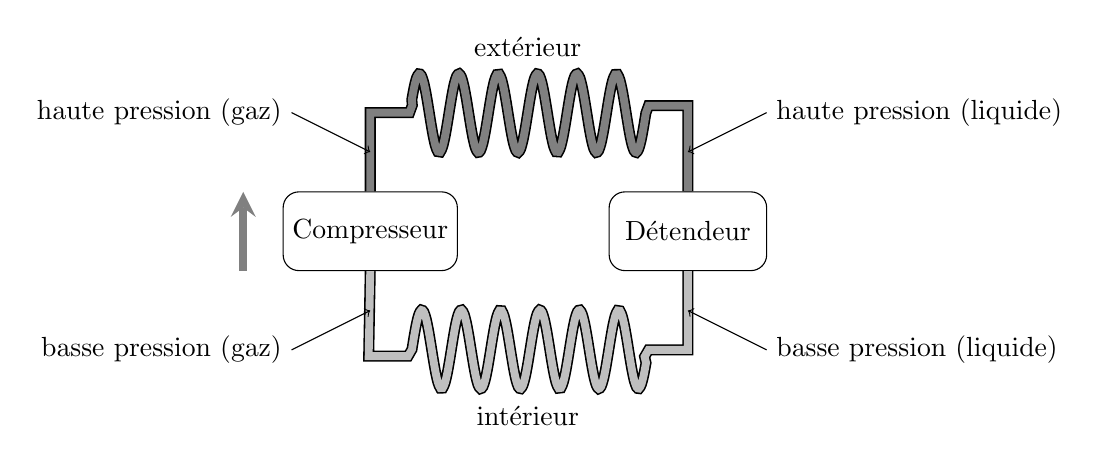
\begin{tikzpicture}
    %tikz thermo
    \node[rectangle, draw, minimum width=2cm, minimum height=1cm, rounded corners=2mm](C) at (0,0) {Compresseur};
    \draw[ 
          line width = 1mm,
          gray,preaction={draw, line width=1.4mm, black},
          ](C.north) -- ++(0,1) coordinate(A);
    \draw[
          line width = 1mm,
          gray,
          preaction={draw, line width=1.4mm, black},
          ] (C.north) -- ++(0,1) --++(0.5,0) --++(70:0.1) --plot[smooth,samples=100,domain=20:6*360] (0.5+(\x/360/2,{1.5+0.5*sin(\x)}) -- ++(70:0.1) --++(0.5,0) coordinate (T1) -- (C.north-|T1) coordinate(B);
    \node[rectangle, draw, minimum width=2cm, minimum height=1cm, rounded corners=2mm,below](D) at (B) {Détendeur};
    \draw[
          line width = 1mm,
          gray!50,
          preaction={draw, line width=1.4mm, black},
          ] (D.south) -- ++(0,-1) --++(-0.5,0) --++(-120:0.1) --plot[smooth,samples=100,domain=20:6*360] (3.53-\x/360/2,{-1.5-0.5*sin(\x)}) -- ++(-120:0.1) --++(-0.5,0) -- (C.south) coordinate();
    \draw[-stealth, line width=1mm, gray] (C.west) ++(-0.5,-0.5) -- ++(0,1); 
    \draw (2, 2.1) node[above]{extérieur};
    \draw (2, -2.1) node[below]{intérieur};
    \draw[<-] (D.north) ++(0, 0.5) -- ++(1, 0.5) node[right]{haute pression (liquide)};
    \draw[<-] (C.north) ++(0, 0.5) -- ++(-1, 0.5) node[left]{haute pression (gaz)};
    \draw[<-] (D.south) ++(0, -0.5) -- ++(1, -0.5) node[right]{basse pression (liquide)};
    \draw[<-] (C.south) ++(0, -0.5) -- ++(-1, -0.5) node[left]{basse pression (gaz)};
  \end{tikzpicture}
  \captionof{figure}{Principe de fonctionnement d'un réfrigérateur.}
\end{center}
Nous modéliserons le système de la manière suivante :
\begin{itemize}
  \item Le système thermodynamique étudié est une masse $m$ de fluide frigorifique ;
  \item le milieu extérieur est une source chaude à la température $T_c$ qui fournit une chaleur $Q_c<0$ au système (c'est le fluide qui réchauffe l'extérieur) ;
  \item le milieu intérieur est une source froide à la température $T_f$ qui fournit une chaleur $Q_f>0$  au système ;
  \item le compresseur fournit un travail $W>0$ au système. 
\end{itemize}

\begin{center}
  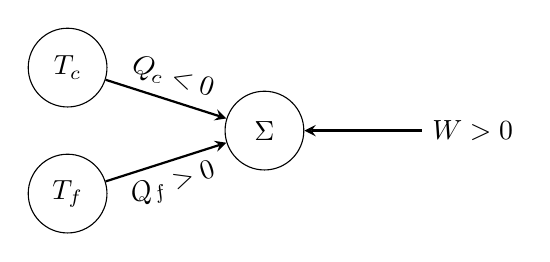
\begin{tikzpicture}
    %tikz thermo
    \node[circle, draw, minimum width=1cm] at (-2.5, 0.8) (Tc){ $T_c$ };
    \node[circle, draw, minimum width=1cm] at (-2.5, -0.8) (Tf){ $T_f$ };
    \node[circle, draw, minimum width=1cm] at (0,0) (S){ $\Sigma$ };
    \draw[-stealth, thick] (Tc) -- node[above,sloped]{ $Q_c<0$ }(S);
    \draw[-stealth, thick] (Tf) -- node[below, sloped]{ $Q_f>0$ }(S);
    \draw[stealth-, thick] (S) --  ++(2, 0)node[right]{ $W>0$ };
  \end{tikzpicture}
\captionof{figure}{Modélisation du réfrigérateur.}
\end{center}

C'est un \textbf{récepteur ditherme}, il reçoit du travail du milieu extérieur et échange de la chaleur avec deux thermostats. 
\section{Résultats théoriques, théorème de Carnot}%
\label{sec:resultats_theoriques_theoreme_de_carnot}
\subsection{Moteur ditherme}%
\label{sub:moteur_ditherme}

On étudie le moteur ditherme suivant sur un cycle. L'état final du système $\Sigma$ est identique à son état initial.

\begin{center}
  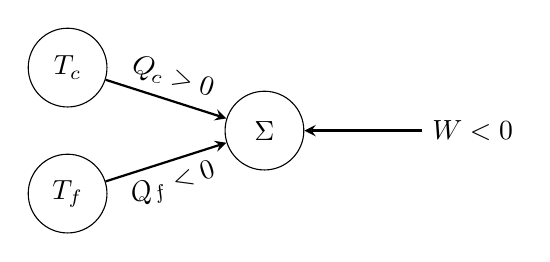
\begin{tikzpicture}
    %tikz thermo
    \node[circle, draw, minimum width=1cm] at (-2.5, 0.8) (Tc){ $T_c$ };
    \node[circle, draw, minimum width=1cm] at (-2.5, -0.8) (Tf){ $T_f$ };
    \node[circle, draw, minimum width=1cm] at (0,0) (S){ $\Sigma$ };
    \draw[-stealth, thick] (Tc) -- node[above,sloped]{ $Q_c>0$ }(S);
    \draw[-stealth, thick] (Tf) -- node[below, sloped]{ $Q_f<0$ }(S);
    \draw[stealth-, thick] (S) --  ++(2, 0)node[right]{ $W<0$ };
  \end{tikzpicture}
\captionof{figure}{Moteur ditherme.}
\end{center}

Nous allons chercher à déterminer le rendement $\eta$ de ce moteur, défini comme
\begin{equation}
  \eta = \frac{\text{travail fourni}}{\text{énergie consommée}} = \frac{-W}{Q_c}
\end{equation}
L'énergie consommée est $Q_c$ car dans un moteur ditherme c'est toujours l'énergie prise à la source chaude qui \emph{coûte}, elle coûte par exemple du charbon pour faire avancer une locomotive, de l'uranium pour faire fonctionner une centrale nucléaire...

L'application du premier principe sur un cycle donne
\begin{equation}
  \Delta U = 0 = W + Q = W + Q_c + Q_f
\end{equation}

L'application du second principe sur un cycle donne
\begin{equation}
  \Delta S = 0 = S_\text{créée} + S_{\text{éch.}} = \underbrace{S_\text{créée}}_{\geq 0} + \frac{Q_c}{T_c} + \frac{Q_f}{T_f} \geq \frac{Q_c}{T_c} + \frac{Q_f}{T_f}
\end{equation}
On en déduit l'inégalité de Clausius :
\begin{equation}
  \frac{Q_c}{T_c} + \frac{Q_f}{T_f}\leq 0
\end{equation}
Il y a égalité dans le cas d'une transformation réversible. On peut donc écrire le rendement du moteur comme
\begin{equation}
  \eta=\frac{-W}{Q_c} = \frac{Q_c+Q_f}{Q_c} = 1+\frac{Q_f}{Q_c}
\end{equation}
Or,
\begin{equation}
  \frac{Q_f}{T_f}\leq \frac{Q_c}{T_c} \quad \Leftrightarrow \quad \frac{Q_f}{Q_c}\leq \frac{-T_f}{T_c}
\end{equation}
Et on en déduit le théorème de Carnot qui donne le rendement théorique maximum pour un moteur ditherme 
\begin{loi}{Théorème de Carnot}
Le rendement maximum d'un moteur ditherme est 
\begin{equation}
  \eta_\text{max}= 1-\frac{T_f}{T_c}\, ,  
\end{equation}
et il est atteint lorsque les transformations sont réversibles.
\end{loi}
 On en déduit que tous les moteurs dithermes réversibles ont exactement le même rendement.

 \begin{application}
   Dans une centrale nucléaire, le générateur de vapeur a une température $T_c=\SI{300}{\celsius}$, la source froide est à la température $T_f=\SI{25}{\celsius}$. D'après le théorème de Carnot, le rendement maximum de la centrale est
   \begin{equation}
     \eta_\text{max}=1-\frac{T_f}{T_c} \approx \luaexec{SI(100*(1-293/573), 0, "\\percent")}
   \end{equation}
   En pratique, les centrales nucléaires ont un rendement de l'ordre de \SI{30}{\percent}
 \end{application}
 Le rendement d'un moteur à essence est de l'ordre de \SI{30}{\percent} et le rendement d'un moteur diesel de l'ordre de \SI{50}{\percent}.

 \subsection{Réfrigérateur}%
 \label{sub:refrigerateur}

La modélisation du frigo est la même que celle du moteur ditherme, seuls les signes des échanges d'énergie changent.
 
\begin{center}
  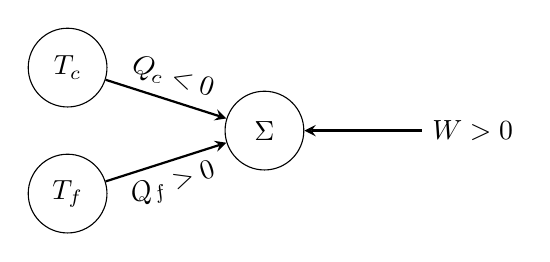
\begin{tikzpicture}
    %tikz thermo
    \node[circle, draw, minimum width=1cm] at (-2.5, 0.8) (Tc){ $T_c$ };
    \node[circle, draw, minimum width=1cm] at (-2.5, -0.8) (Tf){ $T_f$ };
    \node[circle, draw, minimum width=1cm] at (0,0) (S){ $\Sigma$ };
    \draw[-stealth, thick] (Tc) -- node[above,sloped]{ $Q_c<0$ }(S);
    \draw[-stealth, thick] (Tf) -- node[below, sloped]{ $Q_f>0$ }(S);
    \draw[stealth-, thick] (S) --  ++(2, 0)node[right]{ $W>0$ };
  \end{tikzpicture}
\captionof{figure}{Modélisation du réfrigérateur.}
\end{center}
%
Cette fois, on définit l' \textbf{efficacité} du frigo comme 
\begin{equation}
  e = \frac{Q_f}{W}
\end{equation}
L'application du premier principe donne comme dans le cas précédent
\begin{equation}
  \Delta U = 0 = W + Q_c + Q_f \Leftrightarrow W=-(Q_c + Q_f)\, .
\end{equation}
Le second principe donne à nouveau l'inégalité de Clausius
\begin{equation}
 \frac{Q_c}{T_c}+ \frac{Q_f}{T_f}\leq 0  
\end{equation}
donc 
\begin{equation}
  e=-\frac{Q_f}{Q_c+Q_f}=-\frac{1}{1+\frac{Q_c}{Q_f}}
\end{equation}
or
\begin{equation}
  \frac{Q_c}{T_c}\leq -\frac{Q_f}{T_f} \Leftrightarrow \frac{Q_c}{Q_f} \leq - \frac{T_c}{T_f} \Leftrightarrow \frac{T_c}{T_f}-1 \leq -1-\frac{Q_c}{Q_f}
\end{equation}
et on en déduit finalement que 
\begin{eqencadre}
  \eta\leq \frac{1}{\frac{T_c}{T_f}-1}
\end{eqencadre}  
Et à nouveau, l'efficacité maximum est atteinte lorsque le frigo fonctionne de manière réversible.

Pour un frigo réel, avec $T_c=\SI{20}{\celsius}$ et $T_f=\SI{0}{\celsius}$, on trouve $e_\text{max}\approx \luaexec{SI(1/(293/273-1), 0, "")}$. En pratique, l'efficacité d'un frigo réel est de l'ordre de 3. 

\end{document}
\section{Application à une machine thermique réel : le réfrigérateur}%
\label{sec:application_a_une_machine_thermique_reel_le_refrigerateur}

\subsection{Premier principe pour un fluide en écoulement permanent}%
\label{sub:premier_principe_pour_un_fluide_en_ecoulement}

On considère un fluide en écoulement permanent dans un circuit. Nous allons déterminer l'expression de la variation d'enthalpie massique du fluide lorsqu'il passe dans une portion du circuit.

On s'intéresse à l'évolution d'une partie du fluide entre les instants $t$ et $t+\D t$.

\begin{center}
  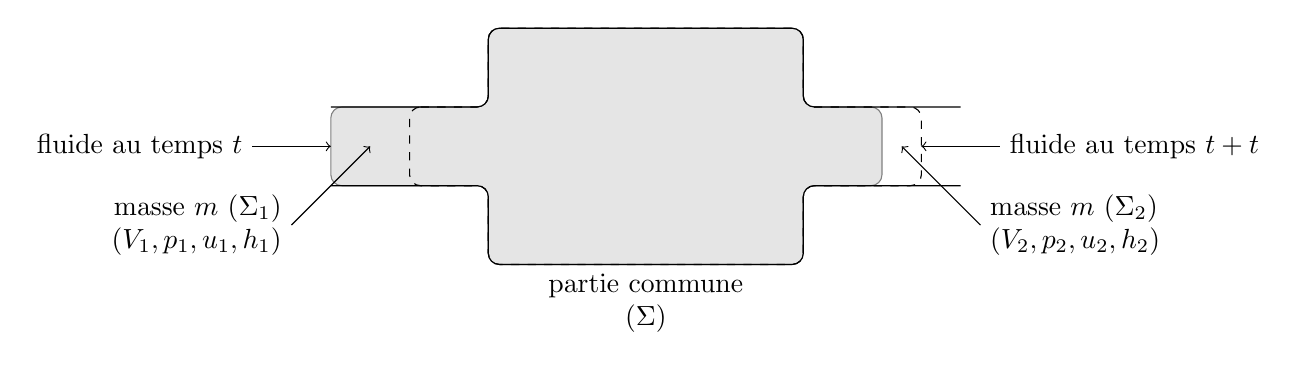
\begin{tikzpicture}
    %tikz thermo
    \fill[rounded corners, gray!20, draw=gray] 
    (0,0.5) -- ++(2,0) -- ++(0,1) -- ++ (4, 0 ) -- ++(0, -1) -- ++(1,0) --
    ++(0,-1) -- ++(-1,0) -- ++(0,-1) -- ++ (-4, 0 ) -- ++(0, 1) -- ++(-2,0) --cycle ; 
    \draw[rounded corners, dashed] (1,0.5) -- ++(1,0) -- ++(0,1) -- ++ (4, 0 ) -- ++(0, -1) -- ++(1.5,0) --
    ++(0,-1) -- ++(-1.5,0) -- ++(0,-1) -- ++ (-4, 0 ) -- ++(0, 1) -- ++(-1,0) --cycle ; 
    \draw[rounded corners] 
    (0,0.5) -- ++(2,0) -- ++(0,1) -- ++ (4, 0 ) -- ++(0, -1) -- ++(2,0) 
    ++(0,-1) -- ++(-2,0) -- ++(0,-1) -- ++ (-4, 0 ) -- ++(0, 1) -- ++(-2,0) ; 

    \draw[<-] (0, 0) -- ++ (-1, 0) node[left]{fluide au temps $t$ };
    \draw[<-] (7.5, 0) -- ++ (1, 0) node[right]{fluide au temps $t+\D t$ };
    \draw (4, -1.5) node[below, align=center]{partie commune\\ ($\Sigma$)};
    \draw[<-] (0.5, 0) -- ++ (-1, -1) node[left, align=right]{masse $\D m$ ($\Sigma_1$) \\ ($\D V_1, p_1, u_1, h_1$)};
    \draw[<-] (7.25, 0) -- ++ (1, -1) node[right, align=left]{masse $\D m$ ($\Sigma_2$)\\ ($\D V_2, p_2, u_2, h_2$) };
  \end{tikzpicture}
\captionof{figure}{fluide en écoulement stationnaire.}
\end{center}

On sépare la conduite en trois parties :
\begin{itemize}
  \item au temps $t$, le fluide occupe les parties $\Sigma_1$ et $\Sigma$. La partie $\Sigma_1$ contient une masse $\D m$  de fluide.
  \item au temps $t+\D t$, le fluide occupe les parties $\Sigma$ et $\Sigma_2$.  Comme l'écoulement est stationnaire, la masse de fluide qui occupe la partie $\Sigma_2$ est aussi $\D m$, car la masse de fluide contenue dans $\Sigma$ doit rester constante, la masse de fluide qui entre dans $\Sigma$ pendant le temps $\D t$ doit être égale à la masse de fluide qui en sort. 
\end{itemize}

On définit les grandeurs suivantes :
\begin{itemize}
  \item Dans la partie $\Sigma_1$, de volume $\D V_1$, la pression est $p_1$, l'énergie interne massique est $u_1$ et l'enthalpie massique est $h_1$ ;
  \item dans la partie $\Sigma_2$, de volume $\D V_2$, la pression est $p_2$, l'énergie interne massique est $u_2$ et l'enthalpie massique est $h_2$. 
\end{itemize}

On considère que l'énergie cinétique macroscopique du fluide ne change pas beaucoup entre l'entrée et la sortie, le premier principe de la thermodynamique donne 
\begin{equation}
  \Delta U = W + Q = W_\text{pression} + W_\text{utile} + Q \, ,
\end{equation}
où $W_\text{pression}$ est le travail des forces de pression et $W_\text{utile}$ est le travail fourni au fluide par d'autres moyens (pièces mobiles dans le système).

Le travail des forces de pression est la somme des travaux des forces de pression en aval et en amont :
\begin{equation}
  W_\text{pression} = p_1 \D V_1 - p_2 \D V_2\, .
\end{equation}  
Par ailleurs, on peut écrire $\Delta U$ comme
\begin{equation}
  \Delta U = U(t+\D t) - U(t) = U(\Sigma) + U(\Sigma_2) - (U(\Sigma) + U(\Sigma_1)) = U(\Sigma_2) - U(\Sigma_1)  
\end{equation}
On a donc
\begin{equation}
  U_2 - U_1 = p_1 \D V_1 -p_2 \D V_2 + W_u + Q \Leftrightarrow \underbrace{(U_2 + p_2 \D V_2)}_{H_2} -\underbrace{(U_1 + p_1 \D V_1)}_{H_1} = W_u + Q \, .
\end{equation}
En divisant par $\D m$, on obtient :
\begin{eqencadre}
  \Delta h = h_2 - h_1 = w_u + q
\end{eqencadre}
où $\Delta h$ est la variation d'enthalpie massique du fluide entre l'entrée et la sortie de la portion de circuit considérée, $w_u$ est le travail massique utile (autre que les forces de pression) fourni au fluide et $q$ la chaleur massique fournie au fluide.

\subsection{Cycle du réfrigérateur}%
\label{sub:cycle_du_refrigerateur}



On étudie un réfrigérateur réel constitué d'un circuit dans lequel circule le fluide réfrigérant : du 1,1,1,2-Tétrafluoroéthane aussi connu sous le nom de R134a. Le cycle subit par le fluide réfrigérant est le suivant :
\begin{itemize}
  \item Compression adiabatique réversible du gaz (dans le compresseur !) depuis un état ($A$ ) $(p_1=\SI{2}{bar}, T_1=\SI{20}{\celsius})$ vers l'état ($B$) $(p_2=\SI{10}{\bar}, T_2)$. Nous déterminerons la température $T_2$ plus tard. 
  \item Le fluide passe dans le condenseur où il se liquéfie à pression constante pour atteindre une température $T_3=\SI{20}{\celsius}$ et l'état ($C$). 
  \item Il passe ensuite dans le détendeur où il subit une détente isenthalpique pour revenir à une pression de \SI{2}{bar} et une température $T_4$, c'est l'état ($D$) . 
  \item Dans l'évaporateur, il subit une transformation isobare qui l'amène à la température $T_5=\SI{5}{\celsius}$ ($E$).
  \item Enfin il subit un échauffement isobare qui le ramène à l'état initial $(p_1=\SI{2}{bar}, T_1=\SI{20}{\celsius})$.
\end{itemize}
On représente le cycle subit dans un \textbf{diagramme enthalpique} (ou diagramme de Mollier, ou diagramme des frigoristes) où on trace la pression du fluide en fonction de son enthalpie massique.  
\begin{center}
  \begin{tikzpicture}
    \begin{axis}[
        width=15cm,
        height=10cm,
        ymin=0.5, 
        ymax=60,
        xmin=1.4e2,
        xmax=5.5e2,
        ymode=log,
        grid=both,
        minor x tick num=4,
        x tick style={black},
        clip mode=individual,
        %clip=false,
        xlabel=Enthalpie massique (\si{\kilo\joule\per\kilo\gram}),
        ylabel=Pression (\si{bar}),
        ]
    %% Isochores
  \begin{luacode}  
  d={1.6667,2.4850,3.7050,5.5241,8.2363,12.2801,18.3093,27.2988,40.7018,60.6855,90.4806,134.9044,201.1392,299.8937,447.1344,666.6667}
  j=1
  \end{luacode} 
  \foreach \i in {0,1,...,5}{
  %\foreach \i in {0,1}{
      \addplot[mark=none,thin, green] table[x index=0, y index=1] {data/R134a/isochore\i.csv} coordinate (A);
      \draw[green] (A) -- ++(6mm, 6mm) node[right, rotate=45, green]{\tiny \luaexec{tex.print(string.format("$\\num{\%.2f}$",1/d[j]));j=j+1}};
      }
  \foreach \i in {6,7,...,12}{
  %\foreach \i in {0,1}{
      \addplot[mark=none,thin, green] table[x index=0, y index=1] {data/R134a/isochore\i.csv} coordinate (A);
      \draw[green] (A) -- ++(6mm, 6mm) node[right, rotate=45, green]{\tiny \luaexec{tex.print(string.format("$\\num{\%.3f}$",1/d[j]));j=j+1}};
      }
  \foreach \i in {13,14,...,15}{
  %\foreach \i in {0,1}{
      \addplot[mark=none,thin, green] table[x index=0, y index=1] {data/R134a/isochore\i.csv} coordinate (A);
      \draw[green] (A) -- ++(6mm, 6mm) node[right, rotate=45, green]{\tiny \luaexec{tex.print(string.format("$\\num{\%.4f}$",1/d[j]));j=j+1}};
      }

      %%Isentropiques
\luaexec{entr=0.8}
 \foreach \i in {0,1,...,15}{
      \addplot[mark=none,thin, blue] table[x index=0, y index=1] {data/R134a/isentropique\i.csv} coordinate (A);
      \draw[blue] (A) -- ++(2mm, 2mm) node[right,rotate=45,blue, fill=white, inner sep=0]{\tiny \luaexec{tex.print(string.format("$\\num{\%.2f}$",entr));entr=entr+0.1}};
      }

      %Isotitres
      \luaexec{i=1}
      \foreach \i in {1,2,...,9}{
      \addplot[name path=isotitre, mark=none,thin, gray] table[x index=0, y index=1] {data/R134a/isotitre\i.csv};
      \path[name path=p] (axis cs:140,1.4) -- (axis cs:400,1.4);
      \draw[name intersections={of=isotitre  and p}] (intersection-1) node[gray,fill=white, rotate=70] {\tiny \luaexec{tex.print(string.format("\\num{\%.2f}",i/10));i=i+1}};
      node[pos=0.4, gray, sloped, fill=white]{\tiny 2.43};
      }
      \addplot[mark=none, thick, name path=ebul,clip=true] table[x index=0, y index=1] {data/R134a/isotitre0.csv};
      \addplot[mark=none, thick, name path=rosee,clip=true] table[x index=0, y index=1] {data/R134a/isotitre10.csv};
      
      %Isothermes
      \luaexec{temp=-40}
      \foreach \i in {0,1,...,14}{
      \addplot[mark=none,thin, red] table[x index=0, y index=1] {data/R134a/isothermes\i.csv} node[pos=1, left, red, fill=white, inner sep=0](T){\tiny \luaexec{tex.print(string.format("\\num{\%d}",temp))}};
      \path[name path=p] (T.east) -- ++(-300, 0);
      \draw[name intersections={of=p and ebul}, red] (intersection-1) -- ++(0.2cm, 0) node[right, fill=white, inner sep=0]{\tiny \luaexec{tex.print(string.format("\\num{\%d}",temp));temp=temp+10}} (intersection-1) -- ++(0, 0.2cm) ;
      }
      \foreach \i in {15,16,...,23}{
      \addplot[mark=none,thin, red] table[x index=0, y index=1] {data/R134a/isothermes\i.csv} ;
      }

      %Légende
      \draw (axis description cs:0,1) ++(10mm,8mm) node[right, blue](LS){\tiny Isentropiques (\si{\joule\per\kelvin\per\kilo\gram})};
      \draw (axis description cs:1,0.5) ++(10mm,0mm) node[below, green, rotate=90]{\tiny Isochores (\si{\cubic\meter\per\kilo\gram})};
      \draw (LS.east) node[right, red]{\tiny Isothermes (\si{\celsius})};


      \coordinate (A) at (axis cs:418, 2);
      \draw[fill] (A) circle(1pt) node[below right]{$A$};
      \coordinate (B) at (axis cs:457.17, 10);
      \draw[fill] (B) circle(1pt) node[above right]{$B$};
      \coordinate (C) at (axis cs:227.88, 10);
      \draw[fill] (C) circle(1pt) node[above left]{$C$};
      \coordinate (D) at (axis cs:227.88, 2);
      \draw[fill] (D) circle(1pt) node[above left]{$D$};
      \coordinate (E) at (axis cs:405.9, 2);
      \draw[fill] (E) circle(1pt) node[below]{$E$};
      \draw[thick](A) -- (B) -- (C) -- (D) -- (E) -- (A);
    \end{axis}
  \end{tikzpicture}
\end{center}

Sur ce diagramme, on a aussi représenté des isothermes (en rouge), des isentropiques (en bleu), des isochores (en vert) et des isotitres (en gris). On reconnait une forme similaire à celle du diagramme de Clapeyron avec le liquide à gauche, la vapeur à droite et un mélange liquide/vapeur sous la cloche. 

Dans la partie liquide, les isothermes sont quasiment verticales, on ne les a donc pas représentées.

Voici quelques indications sur la construction et la lecture de ce diagramme :
\begin{itemize}
  \item On commence par placer le point $A$ à l'intersection de l'isotherme à \SI{20}{\celsius} et de l'isobare à \SI{2}{\bar}.

  \item On arrive au point $B$ en suivant une isentropique jusqu'à la pression de \SI{10}{\bar}. On lit alors sur le diagramme que la température du fluide est autour de \SI{75}{\celsius}.

  \item On arrive ensuite au point $C$ en suivant l'isobare à \SI{10}{\bar} jusqu'à rencontrer l'isotherme à \SI{20}{\celsius} ; elle se trouve à la verticale du point noté \SI{20}{\celsius} dans la partie liquide. On remarque qu'au cours de cette transformation, le gaz commence par refroidir, puis il est totalement liquéfié pour devenir totalement liquide à \SI{40}{\celsius} et enfin le liquide est refroidi jusqu'à \SI{20}{\celsius}. On dit que le liquide est \emph{sous-refroidi}.

  \item Pour atteindre le point $D$, on suit une isenthalpique (verticale) jusqu'à \SI{2}{\bar}. On observe qu'au point $D$, \SI{20}{\percent} de la masse du fluide est sous forme gazeuse. La température du fluide est de \SI{-10}{\celsius}.

  \item On arrive au point $E$ en suivant l'isobare à \SI{2}{\bar} jusqu'à rencontrer l'isotherme à \SI{5}{\celsius}.

  \item On revient au point $A$ en suivant l'isobare à \SI{2}{\bar}.
\end{itemize}

On peut aussi utiliser ce diagramme pour déterminer l'efficacité du frigo. Notons $D_m$ le débit massique de fluide dans le circuit. Lors de la phase de compression ($AB$), on peut écrire le premier principe pour un fluide en écoulement :
\begin{equation}
  \Delta h  = w_u + q = w_u \quad \text{car compression adiabatique}
\end{equation}  
On en déduit que le travail massique fourni par le compresseur est 
\begin{equation}
  w_u = \Delta h = h_B-h_A = \SI{38}{\kilo\joule\per\kilo\gram}
\end{equation}

En appliquant le premier principe lors du passage dans l'évaporateur, entre $D$ et $E$, on trouve la transfert thermique massique reçu par le fluide de l'intérieur du frigo :
\begin{equation}
  q_f = \Delta h = h_E-h_D = \SI{175}{\kilo\joule\per\kilo\gram}
\end{equation}

On peut en déduire l'efficacité énergétique du frigo, aussi appelé \emph{coefficient de performance} :
\begin{equation}
  e=\frac{q_f}{w_u} \approx \num{4.6}
\end{equation}



\end{document}
